\begin{figure}[tb]
    \centering
    \begin{minipage}{.5\linewidth}
      \centering
      \begin{tikzpicture}[
            box/.style={rectangle, draw, rounded corners, align=center, minimum height=10mm, minimum width=16mm},
            leaf/.style={circle, draw, align=center, minimum size=10mm},
            line/.style={-latex}
        ]
        
        % Root node
        \node [box] (root) {$x_1 < 0.7$};
    
        % Level 1 nodes
        \node [box, below=1cm of root, xshift=-2cm] (left) {$x_2 < 0.6$};
        \node [leaf, below=1cm of root, xshift=2cm] (h1) {$h_1$};
    
        % Level 2 nodes
        \node [leaf, below=1cm of left, xshift=-1cm] (h2) {$h_2$};
        \node [leaf, below=1cm of left, xshift=1cm] (h3) {$h_3$};
    
        % Draw edges with labels
        \draw[line] (root) -- (left) node[midway, above left] {Yes};
        \draw[line] (root) -- (h1) node[midway, above right] {No};
        \draw[line] (left) -- (h2) node[midway, above left] {Yes};
        \draw[line] (left) -- (h3) node[midway, above right] {No};
    
        \end{tikzpicture}
    \end{minipage}%
    \begin{minipage}{.5\linewidth}
      \centering
      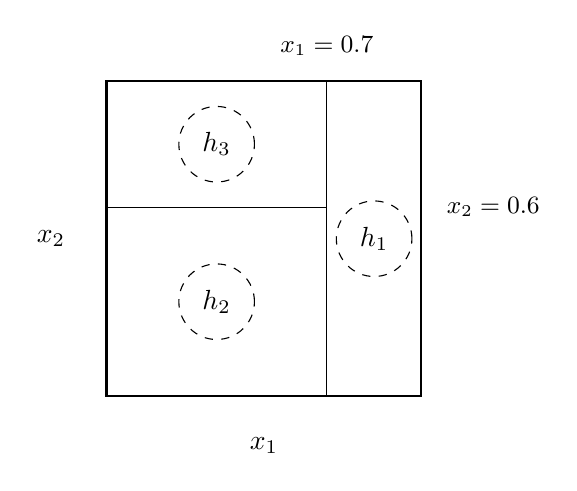
\begin{tikzpicture}[scale=4] % Increase scale for a larger square
            % Define the unit square
            \draw[thick] (0, 0) rectangle (1, 1);
            
            % Vertical line at x1 = 0.4
            \draw[thin] (0.7, 0) -- (0.7, 1) ;
            
            % Horizontal line at x2 = 0.7
            \draw[thin] (0, 0.6) -- (0.7, 0.6);
            
            % Labels for axes
            \node[below] at (0.5, -0.1) {$x_1$};
            \node[left] at (-0.1, 0.5) {$x_2$};
    
            % Splitting variables of the partition
            \node[right] at (1.05, 0.6)  {\small{$x_2 = 0.6$}};
            \node[above] at (0.7, 1.05)  {\small{$x_1 = 0.7$}};
            
            % Step heights
            \node at (0.85, 0.5) {$h_1$};
            \node at (0.35, 0.3) {$h_2$};
            \node at (0.35, 0.8) {$h_3$};
    
            % Circles arounnd 
            \draw[dashed] (0.85, 0.5) circle [radius=0.12];
            \draw[dashed] (0.35, 0.3) circle [radius=0.12];
            \draw[dashed] (0.35, 0.8) circle [radius=0.12];
            
        \end{tikzpicture}
    \end{minipage}
    \caption{Example of a decision tree with the corresponding partition of the covariate space $[0,1]^2$ and the associated step heights $\H = \{h_1, h_2, h_3\}$.}
    \label{ExampleTree}
\end{figure}

